\documentclass[a4paper,12pt]{article}
\usepackage{amsmath}
\usepackage{graphicx}
\usepackage{listings}
\usepackage{caption}
\usepackage{hyperref}
\usepackage{booktabs}
\usepackage{pgfplots} % For including plots
\usepackage{ragged2e}
\usepackage[dvipsnames]{xcolor}
\usepackage{float}
\usepackage{geometry}
\usepackage{wrapfig} % Required for wrapping text around figures
\geometry{margin=2.5cm} % <-- Set all margins to 2.5cm. Change as needed.
\usepackage[most]{tcolorbox}

\usepackage{graphicx} % For including images
\usepackage{caption}    % For customized captions
\usepackage{subcaption} % For subfigures (multiple images in one figure environment)
\usepackage{float}      % For more control over float placement, e.g., [H]
% Adjust geometry if needed for better page layout with many images
% \usepackage[margin=2.5cm]{geometry}


\hypersetup{
    hidelinks
}


\usepackage{xcolor}

\definecolor{codegreen}{rgb}{0,0.6,0}
\definecolor{codegray}{rgb}{0.5,0.5,0.5}
\definecolor{codepurple}{rgb}{0.58,0,0.82}
\definecolor{backcolour}{rgb}{0.95,0.95,0.92}

\tcbset{
    frame code={},
    center title,
    left=0pt,
    right=0pt,
    top=0pt,
    bottom=0pt,
    colback=backcolour,
    colframe=white,
    width=\dimexpr\textwidth\relax,
    enlarge left by=0mm,
    boxsep=5pt,
    arc=0pt,outer arc=0pt,
    }



\lstdefinestyle{mystyle}{
    backgroundcolor=\color{backcolour},   
    commentstyle=\color{Green},
	keywordstyle=\color{blue},
	numberstyle=\tiny\color{Black},
	stringstyle=\color{YellowOrange},
    basicstyle=\ttfamily\footnotesize,
    breakatwhitespace=false,         
    breaklines=true,                 
    captionpos=b,                    
    keepspaces=true,                 
    numbers=left,                    
    numbersep=5pt,                  
    showspaces=false,                
    showstringspaces=false,
    showtabs=false,                  
    %tabsize=2
}

\lstset{style=mystyle}

\usepackage{graphicx} % Required for inserting images

\title{Artificial Intelligence and Machine Learning -\\Reinforcement Learning in the CliffWalking environment}
\date{}
\author{Authors:\\Alessandro Rocchi\\Onorio Iacobelli}

\begin{document}

\maketitle

\tableofcontents

\newpage

\section{Introduction}
In this Machine Learning project we will focus on the subject of Reinforcement Learning applied to the "Cliff Walking" environment. The goal of the agent is to reach a specified location, by moving in the four directions without falling down the cliff. This problem represents a fundamental challenge in Reinforcement Learning, combining elements of exploration/exploitation tradeoff, temporal credit assignment and policy optimization. This environment provides an excellent testbed for comparing different Reinforcement Learning approaches, in particular tabular Q-learning and Deep Q-Networks (DQN).
\vspace{0,5cm}\\
Our implementation explores both classical tabular methods, suitable for discrete state spaces and modern deep learning approaches that can handle more complex scenarios. Trough extensive experimentation and hyperparameter tuning, we demonstrate how different choices and configurations impact learning performance and convergence behavior. 
\section{Reinforcement Learning}
Reinforcement Learning is a branch of machine learning focused on decision making trough interaction with the environment. Unlike supervised learning, where the correct outputs are given for training, in Reinforcement Learning the agent must discover the optimal behavior by trial and error, guided only by rewards. Formally, Reinforcement Learning is often modeled as a Markov Decision Process (MDP), defined by states, actions, transition probabilities and rewards. The agent's goal is to learn a policy, a mapping from states to actions, that maximizes the expected cumulative reward over time.
\vspace{0,5cm}\\
The core components of a Markov Decision Process are:
\begin{itemize}
    \item \textbf{Agent}: the learner or decision-maker that interacts with the environment. In our case this is the entity navigating the cliff walking grid.
    \item \textbf{Environment}: the external system that the agent interacts with. For cliff walking, this includes the grid world, cliff locations, and reward structure.
    \item \textbf{State (S)}: a representation of the current situation in the environment. In cliff walking, this is the agent's current position in the grid.
    \item \textbf{Action (A)}: the choices available to the agent at any given state.
    \item \textbf{Reward (R)}: the feedback signal from the environment indicating how good or bad the last action was. Rewards guide the learning process.
    \item \textbf{Policy ($\pi$)}: the agent's strategy for choosing actions given states. This can be deterministic (always choose the same action in a given state) or stochastic (choose actions according to a probability distribution).
    \item \textbf{$\delta(s'|s,a)$}: the probability distribution over the transitions.
\end{itemize}
The Reinforcement Learning process follows a continuous loop:
\begin{enumerate}
    \item Observe the current state of the environment
    \item Select an action based on the current policy
    \item Execute the action in the environment
    \item Receive a reward and observe the new state
    \item Update the policy based on the experience
    \item Repeat until learning converges or a stopping criterion is met
\end{enumerate}
One of the fundamental challenges in Reinforcement Learning is balancing \textbf{exploration} (trying new actions to discover potentially better strategies) with \textbf{exploitation} (using known good actions to maximize rewards). This balancing is crucial because too much exploration can lead to the agent wasting time on suboptimal actions, on the other hand with too little exploration the agent may get stuck in a local optimum and never discover the best strategy.
\subsection{Q-Learning}
Q-Learning is a model-free Reinforcement Learning algorithm that learns the quality of actions, telling the agent what actions to take under what circumstances. The "Q" stands for quality, representing the expected future reward for taking a specific action in a specific state.\\ The \textbf{Q-function} Q(s,a) represents the expected cumulative reward when taking action 'a' in state 's' and then following the optimal policy. The learning process involves iteratively updating these Q-values using the Bellman equation:
\begin{figure}[H]
    \centering
    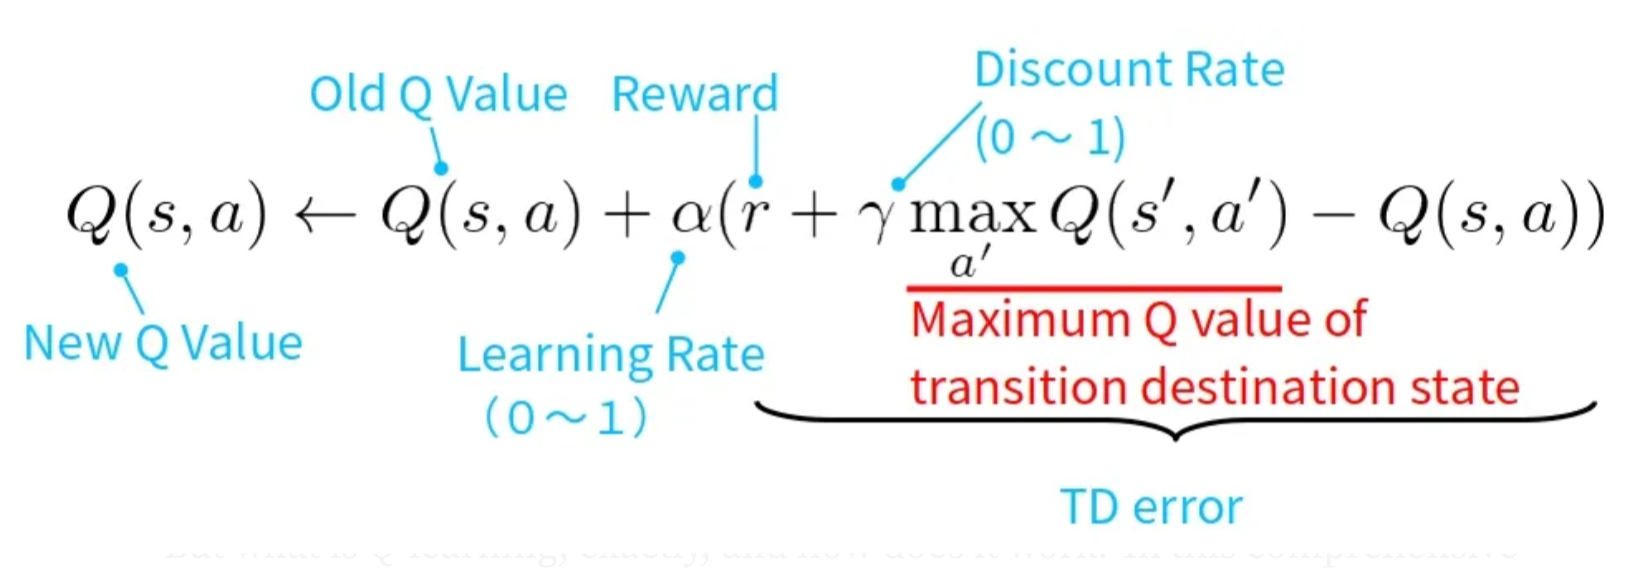
\includegraphics[scale=0.5]{bellman.png}
\end{figure}
Where:
\begin{itemize}
    \item \textbf{$\alpha$ (alpha)}: learning rate controlling how quickly new information overrides old information
    \item \textbf{r}: immediate reward received
    \item \textbf{$\gamma$ (gamma)}: discount factor determining the importance of future rewards
    \item \textbf{s'}: next state after taking action 'a' in state 's'
\end{itemize}
\textbf{Tabular Q-Learning} maintains explicit Q-values for every (state, actions) pair in a lookup table. This approach works well for environments with small, discrete state and action spaces but becomes impractical as the state space grows.
\vspace{0,5cm}\\
\textbf{Deep Q-Networks (DQN)} use neural networks to approximate the Q-function, enabling the handling of large or continuous state spaces. Instead of storing individual Q-values, the network learns to map states to Q-values for all possible actions.
\vspace{0,5cm}\\
To balance exploration and exploitation, we implement an epsilon-greedy policy:
\begin{itemize}
    \item With probability \textbf{$\varepsilon$ (epsilon)}: choose a random action (exploration)
    \item With probability \textbf{1-$\varepsilon$}: choose the action with the highest Q-value (exploitation)
\end{itemize}
The epsilon value starts high (encouraging exploration) and gradually decreases (shifting toward exploitation) as learning progresses.
\section{Environment}
The Cliff Walking environment is part of the Toy Text environments which contains general information about the environment. It involves crossing a grid world from start to goal while avoiding falling off a cliff.
\begin{figure}[H]
    \centering
    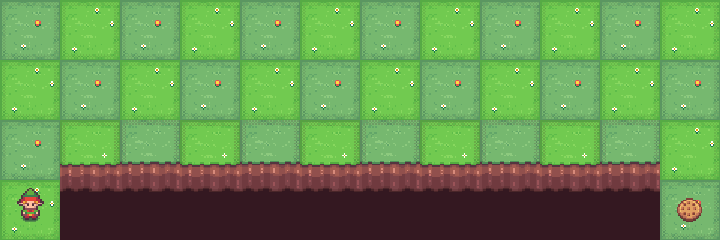
\includegraphics[scale=0.7]{cliff_walking.png}
\end{figure}
\subsection{Description}
The game starts with the player at location [3, 0] of the 4x12 grid world with the goal located at [3, 11]. If the player reaches the goal the episode ends.
\vspace{0,5cm}\\
A cliff runs along [3, 1..10]. If the player moves to a cliff location it returns to the start location.
\vspace{0,5cm}\\
The player makes moves until they reach the goal.
\subsection{Action Space}
The action shape is (1,) in the range \{0, 3\} indicating which direction to move the player.
\begin{itemize}
    \item 0: Move up
    \item 1: Move right
    \item 2: Move down
    \item 3: Move left
\end{itemize}
Actions that would move the agent outside the grid boundaries result in no movement (the agent stays in the same position).
\subsection{Observation Space}
There are 3 x 12 + 1 possible states. The player cannot be at the cliff, nor at the goal as the latter results in the end of the episode. What remains are all the positions of the first 3 rows plus the bottom-left cell.
\vspace{0,5cm}\\
The observation is a value representing the player’s current position as current\_row * ncols + current\_col (where both the row and col start at 0).\\For example, the starting position can be calculated as follows: 3 * 12 + 0 = 36.
\vspace{0,5cm}\\
The observation is returned as an int().
\subsection{Reward}
The reward system is designed to encourage finding the shortest safe path while severely penalizing dangerous moves:
\begin{itemize}
    \item \textbf{Standard step}: -1 reward (encourages shorter paths)
    \item \textbf{Falling off cliff}: -100 reward + episode termination
    \item \textbf{Reaching goal}: 0 reward + episode termination
\end{itemize}
This reward structure creates an interesting dilemma: the shortest path (along the cliff edge) is risky but potentially more rewarding if executed perfectly, while the safe path (around the cliff) is longer but more reliable.
\vspace{0,5cm}\\
The episode terminates when the Agent reaches the goal position, falls of the cliff or the episode can exceeds maximum step limit.
\section{Implementation}
Our approach to solving the Cliff Walking problem implements and compares two fundamental reinforcement learning methodologies: Tabular Q-Learning and Deep Q-Networks (DQN). This comparison allows us to understand the strengths and limitations of each approach while demonstrating how different choices affect learning performance.
\vspace{0,5cm}\\
Both implementations use the code Q-Learning update rule, which is an off-policy temporal difference learning method.
$$Q(s,a) \leftarrow Q(s,a) + \alpha \big[r + \gamma \max_{a'} Q(s',a') - Q(s,a)\big]$$
This update rule is off-policy, meaning it learns about the optimal policy while following a potentially different policy (epsilon-greedy). This property makes Q-learning robust and widely applicable.
\subsection{Framework}
Our solution utilizes the following Python libraries:
\begin{itemize}
    \item \textbf{Gymnasium}: standard Reinforcement Learning environment interface
    \item \textbf{NumPy}: efficient numerical computations for tabular methods
    \item \textbf{PyTorch}: deep learning framework for DQN implementation
    \item \textbf{Matplotlib}: visualization of learning curves and performance metrics
\end{itemize}
The modular design allows easy experimentation with different hyperparameters and direct comparison between approaches under identical conditions.
\subsection{Tabular Q-Learning Implementation Details}
The algorithm follows the standard Q-Learning approach but is tailored for the Cliff Walking environment.
\subsubsection{Q-Table Initialization}
The Q-table is initialized with zeros. Its shape corresponds to the number of states and the number of possible actions in the environment:
\begin{lstlisting}[language=Python]
n_states = env.observation_space.n
n_actions = env.action_space.n
Q = np.zeros((n_states, n_actions))
\end{lstlisting}
\subsubsection{Training Loop}
For each episode, the environment is reset and the agent interacts with it until termination.
\begin{lstlisting}[language=Python]
def train_tabular_q(env):
    episodes = config.TAB_EPISODES
    alpha = config.TAB_ALPHA
    gamma = config.TAB_GAMMA
    epsilon = config.TAB_EPSILON
    epsilon_decay = config.TAB_EPSILON_DECAY
    min_epsilon = config.TAB_MIN_EPSILON

    n_states = env.observation_space.n
    n_actions = env.action_space.n
    Q = np.zeros((n_states, n_actions))

    rewards, epsilon_history, td_errors = [], [], []

    for ep in trange(episodes, desc="Training Tabular Q-learning"):
        state, _ = env.reset()
        done = False
        ep_reward = 0
        ep_td_errors = []

        while not done:
            if config.RENDER:
                print(env.render())

            if np.random.rand() < epsilon:
                action = env.action_space.sample()
            else:
                action = np.argmax(Q[state])

            next_state, reward, terminated, truncated, _ = env.step(action)
            done = terminated or truncated
            ep_reward += reward

            old_value = Q[state, action]
            best_next = np.max(Q[next_state])
            td_target = reward + gamma * best_next * (not done)
            td_error = td_target - old_value
            Q[state, action] += alpha * td_error

            ep_td_errors.append(abs(td_error))

            state = next_state

            if config.RENDER:
                print(f"State: {state}, Action: {action}, Reward: {reward}, Next state: {next_state}\n---\n")

        rewards.append(ep_reward)
        epsilon_history.append(epsilon)
        td_errors.append(np.mean(ep_td_errors))
        epsilon = max(min_epsilon, epsilon * epsilon_decay)

    print("Training complete")

    return Q, rewards, epsilon_history, td_errors
\end{lstlisting}
\subsubsection{Action Selection ($\varepsilon$-greedy)}
The agent chooses an action using the $\varepsilon$-greedy strategy: with probability $\varepsilon$ it selects a random action (exploration), and otherwise it selects the action with the highest Q-value (exploitation).
\begin{lstlisting}[language=Python]
if np.random.rand() < epsilon:
    action = env.action_space.sample()
else:
    action = np.argmax(Q[state])
\end{lstlisting}
\subsubsection{Environment Step and Q-value Update}
After taking an action, the agent observes the next state and reward. The Q-value is updated using the Temporal Difference (TD) learning rule:
\begin{lstlisting}[language=Python]
old_value = Q[state, action]
best_next = np.max(Q[next_state])
td_target = reward + gamma * best_next * (not done)
td_error = td_target - old_value
Q[state, action] += alpha * td_error
\end{lstlisting}
\subsubsection{Track Metrics}
During the training, the following metrics are stored for later visualization:
\begin{itemize}
    \item Episode reward: cumulative sum of the rewards per episode
    \item Epsilon: exploration rate over time
    \item TD errors: average temporal-difference errors per episode
\end{itemize}
\subsubsection{Epsilon Decay}
At the end of each episode, epsilon is decayed to gradually shift from exploration to exploitation:
\begin{lstlisting}
epsilon = max(min_epsilon, epsilon * epsilon_decay)
\end{lstlisting}
\subsection{Deep Q-Network (DQN) Implementation}
Our DQN implementation uses a neural network to approximate Q-values, enabling more complex function approximation capabilities. The network architecture is configurable trough hyperparameters.
\subsubsection{Network Architecture}
\begin{lstlisting}[language=Python]
class DQN(nn.Module):
    def __init__(self, state_size, action_size):
        super().__init__()
        self.embedding = nn.Embedding(state_size, 16)
        
        layers = []
        input_size = 16
        for _ in range(DQN_HIDDEN_LAYERS):
            layers.append(nn.Linear(input_size, DQN_NODES_PER_LAYER))
            layers.append(nn.ReLU())
            input_size = DQN_NODES_PER_LAYER
            
        layers.append(nn.Linear(input_size, action_size))
        self.net = nn.Sequential(*layers)
    
    def forward(self, x):
        x = self.embedding(x)
        return self.net(x)
\end{lstlisting}
The DQN class defines the neural network used to approximate the Q-function. It possesses the following characteristics:
\begin{itemize}
    \item \textbf{State Embedding}: 16-dimensional embedding layer converts discrete states to dense representations
    \item \textbf{Configurable Depth}: number of hidden layers determined by hyperparameters
    \item \textbf{ReLU Activation}: non-linear activation functions enabling complex function approximation
    \item \textbf{Output Layer}: linear layer producing Q-values for all actions
\end{itemize}
\subsubsection{Training function}
The training function implements the training process of the DQN. It initializes the policy and target networks, sets up the replay buffer, and runs the training loop over episodes. These are the key steps:
\begin{enumerate}
    \item Initialize policy and target networks
    \item Run episodes with $\varepsilon$-greedy action selection
    \item Store transitions in replay buffer
    \item Sample minibatches and perform gradient descent
    \item Update target network periodically
    \item Decay epsilon over time
\end{enumerate}
\begin{lstlisting}[language=Python]
def train_dqn(device, env):
    episodes=config.DQN_EPISODES
    batch_size=config.DQN_BATCH_SIZE
    gamma=config.DQN_GAMMA
    epsilon=config.DQN_EPSILON
    min_epsilon=config.DQN_MIN_EPSILON
    epsilon_decay=config.DQN_EPSILON_DECAY
    target_update_freq=config.DQN_TARGET_UPDATE_FREQ
    grad_update_freq=config.DQN_GRAD_UPDATE_FREQ

    n_states = env.observation_space.n
    n_actions = env.action_space.n
    policy_net = DQN(n_states, n_actions).to(device)

    if config.DEBUG:
        print("DQN architecture:\n", policy_net)
        
    target_net = DQN(n_states, n_actions).to(device)
    target_net.load_state_dict(policy_net.state_dict())
    target_net.eval()

    optimizer = optim.Adam(policy_net.parameters(), lr=1e-3)
    criterion = nn.MSELoss()
    replay_buffer = deque(maxlen=1000)
    step_count = 0

    rewards, epsilon_history, losses = [], [], []

    for ep in trange(episodes, desc="Training DQN"):
        state, _ = env.reset()
        done = False
        ep_reward = 0
        ep_losses = []

        while not done:
            step_count += 1
            s_tensor = torch.tensor([state], device=device)

            if random.random() < epsilon:
                action = env.action_space.sample()
            else:
                with torch.no_grad():
                    action = policy_net(s_tensor).argmax().item()

            next_state, reward, terminated, truncated, _ = env.step(action)
            done = terminated or truncated
            ep_reward += reward

            replay_buffer.append((state, action, reward, next_state, done))
            state = next_state

            if step_count % grad_update_freq == 0 and len(replay_buffer) >= batch_size:
                batch = random.sample(replay_buffer, batch_size)
                states, actions, rewards_batch, next_states, dones = zip(*batch)

                states = torch.tensor(states, device=device)
                next_states = torch.tensor(next_states, device=device)
                actions = torch.tensor(actions, device=device)
                rewards_batch = torch.tensor(rewards_batch, dtype=torch.float32, device=device)
                dones = torch.tensor(dones, dtype=torch.bool, device=device)

                q_values = policy_net(states).gather(1, actions.unsqueeze(1)).squeeze()
                with torch.no_grad():
                    next_q = target_net(next_states).max(1)[0]
                    targets = rewards_batch + gamma * next_q * (~dones)

                loss = criterion(q_values, targets)
                optimizer.zero_grad()
                loss.backward()
                optimizer.step()
                ep_losses.append(loss.item())

        rewards.append(ep_reward)
        epsilon_history.append(epsilon)
        avg_loss = np.mean(ep_losses) if ep_losses else 0
        losses.append(avg_loss)

        epsilon = max(min_epsilon, epsilon * epsilon_decay)

        if ep % target_update_freq == 0:
            target_net.load_state_dict(policy_net.state_dict())

    print("Training complete")

    return policy_net, rewards, epsilon_history, losses
\end{lstlisting}
DQN incorporates Experience Replay Buffer to break temporal correlations and improve sample efficiency:
\begin{lstlisting}[language=Python]
replay_buffer = deque(maxlen=10_000)

# Store experiences
replay_buffer.append((state, action, reward, next_state, done))

# Sample random batch for training
if len(replay_buffer) >= batch_size:
    batch = random.sample(replay_buffer, batch_size)
    # Process batch for network update
\end{lstlisting}
Benefits of Experience Replay:
\begin{itemize}
    \item \textbf{Decorrelated Updates}: reduces harmful correlation between consecutive experiences 
    \item \textbf{Sample Efficiency}: reuses experiences multiple times for training
    \item \textbf{Stable Learning}: smoother gradient updates trough diverse batch sampling
\end{itemize}
\begin{lstlisting}[language=Python]
policy_net = DQN(n_states, n_actions)  # Updated every step
target_net = DQN(n_states, n_actions)  # Updated periodically

# Target network update
if episode % target_update_freq == 0:
    target_net.load_state_dict(policy_net.state_dict())
\end{lstlisting}
Target Network Purpose:
\begin{itemize}
    \item \textbf{Stable Targets}: reduces moving target problem in Q-learning
    \item \textbf{Reduced Correlation}: separates action selection from target value computation
    \item \textbf{Improved Convergence}: more stable learning dynamics
\end{itemize}
Our implementation includes a comprehensive configuration system enabling systematic experimentation
\section{Hyperparameters Description}
\begin{lstlisting}[language=Python]
RANDOM_START = True
SLIPPERY = True
EVALUATION_EPISODES = 1000

# Tabular Q-learning parameters
TAB_ALPHA = 0.1
TAB_GAMMA = 0.99
TAB_EPSILON = 1
TAB_MIN_EPSILON = 0.01
TAB_EPSILON_DECAY = 0.995
TAB_EPISODES = 500

# DQN parameters
DQN_BATCH_SIZE = 64
DQN_GAMMA = 0.99
DQN_EPSILON = 1
DQN_MIN_EPSILON = 0.01
DQN_EPSILON_DECAY = 0.995
DQN_BUFFER_SIZE = 1000
DQN_EPISODES = 500
DQN_TARGET_UPDATE_FREQ = 10
DQN_GRAD_UPDATE_FREQ = 4
DQN_HIDDEN_LAYERS = 2
DQN_NODES_PER_LAYER = 32
\end{lstlisting}
\begin{itemize}
    \item \textbf{RANDOM\_START}: enables random starting positions for each episode instead of always starting from the same state
    \item \textbf{SLIPPERY}: introduces stochasticity in action execution (actions have probability of not executing as intended)
    \item \textbf{EVALUATION\_EPISODES}: number of episodes used to evaluate agent performance after training
    \item \textbf{TAB\_ALPHA} (Learning Rate): controls how much new information overrides old Q-values in updates.
    \item \textbf{TAB\_GAMMA} (Discount Factor): determines importance of future rewards relative to immediate rewards
    \item \textbf{TAB\_EPSILON} (Initial Exploration Rate): starting probability of taking random actions for exploration
    \item \textbf{TAB\_MIN\_EPSILON} (Minimum Exploration Rate): lowest bound for exploration probability
    \item \textbf{TAB\_EPSILON\_DECAY} (Exploration Decay Rate): rate at which exploration decreases per episode
    \item \textbf{TAB\_EPISODES} (Training Episodes): total number of training episodes for Tabular Q-Learning
    \item \textbf{DQN\_BATCH\_SIZE} (Mini-batch Size): number of experiences sampled from replay buffer for each training step
    \item \textbf{DQN\_GAMMA} (Discount Factor): same as tabular version but affects neural network target computation
    \item \textbf{DQN\_EPSILON/DQN\_MIN\_EPSILON/DQN\_EPSILON\_DECAY}: same\\ exploration-exploitation mechanism as tabular version
    \item \textbf{DQN\_BUFFER\_SIZE} (Replay Buffer Size): maximum number of experiences stored in replay buffer
    \item \textbf{DQN\_EPISODES} (Training Episodes): total training episodes for DQN
    \item \textbf{DQN\_TARGET\_UPDATE\_FREQ} (Target Network Update Frequency): how often (in episodes) the target network copies weights from policy network
    \item \textbf{DQN\_GRAD\_UPDATE\_FREQ} (Gradient Update Frequency): how often (in environment steps) to perform network parameter updates
    \item \textbf{DQN\_HIDDEN\_LAYERS} (Network Depth): number of hidden layers in the neural network
    \item \textbf{DQN\_NODES\_PER\_LAYER} (Network Width): number of neurons in each hidden layer
\end{itemize}
\section{Evaluation Framework}
Both algorithms share a common evaluation framework ensuring a fair comparison:
\begin{lstlisting}[language=Python]
MAX_EVAL_STEPS = 500
MAX_CONSECUTIVE_REPEAT = 10  # episode ends if agent repeats a state this many times in a row

def evaluate_agent(device, env, policy_net=None, Q=None, tabular=True, random_start=False):
    episodes = config.EVALUATION_EPISODES

    successes, falls, total_rewards, steps_list = 0, 0, [], []

    agent = "DQN" if not tabular else "Tabular Q-learning"
    if not tabular:
        policy_net.eval()

    for ep in trange(episodes, desc="Evaluating " + agent):
        state, _ = env.reset()
        done, ep_reward, steps = False, 0, 0

        last_state = None
        repeat_count = 0

        while not done and steps < MAX_EVAL_STEPS:
            if config.RENDER:
                print(env.render())

            # Select action
            if tabular:
                action = np.argmax(Q[state])
            else:
                state_tensor = torch.tensor([state], device=device)
                with torch.no_grad():
                    action = policy_net(state_tensor).argmax(dim=1).item()

            next_state, reward, terminated, truncated, _ = env.step(action)
            done = terminated or truncated
            ep_reward += reward
            steps += 1

            if last_state == next_state:
                repeat_count += 1
            else:
                repeat_count = 0
            last_state = next_state

            # Trigger early stop if stuck in a repeated state
            if repeat_count >= MAX_CONSECUTIVE_REPEAT:
                if config.DEBUG:
                    print(f"Stuck in state {next_state} for {MAX_CONSECUTIVE_REPEAT} steps. Ending episode early.")
                break

            state = next_state

            if reward == -100:
                falls += 1
            if done and next_state == (env.observation_space.n - 1):
                successes += 1

        total_rewards.append(ep_reward)
        steps_list.append(steps)

        if steps >= MAX_EVAL_STEPS and config.DEBUG:
            print("Max steps reached, ending episode.")

    if not tabular:
        policy_net.train()

    print(f"Evaluation Results (over {episodes} episodes):")
    print(f"  Success Rate: {successes}/{episodes} ({successes/episodes*100:.1f}%)")
    print(f"  Cliff Falls: {falls}")
    print(f"  Avg Total Reward: {np.mean(total_rewards):.2f}")
    print(f"  Avg Steps per Episode: {np.mean(steps_list):.2f}")
\end{lstlisting}
Evaluation Metrics:
\begin{itemize}
    \item \textbf{Success Rate}: percentage of terminated episodes
    \item \textbf{Cliff Falls}: number of cliff accidents
    \item \textbf{Average Reward}: mean cumulative reward per episode
    \item \textbf{Average Steps}: mean episodes length, indicating path efficiency
\end{itemize}
Given our environment, we want the reward to be as small as possible, since each step taken can produce at best a reward of -1.
\section{Testing}
To validate our implementation we performed various tests on different hyperparameters to simulate different situations.

\subsection{Random start}
By default, the agent starts at position [3,0] but we also tried to make it start at a random position every episode.
Adding random start increases average reward since the agent can start closer to the goal and thus require less steps to reach it.

\begin{figure}[H]
    \centering
    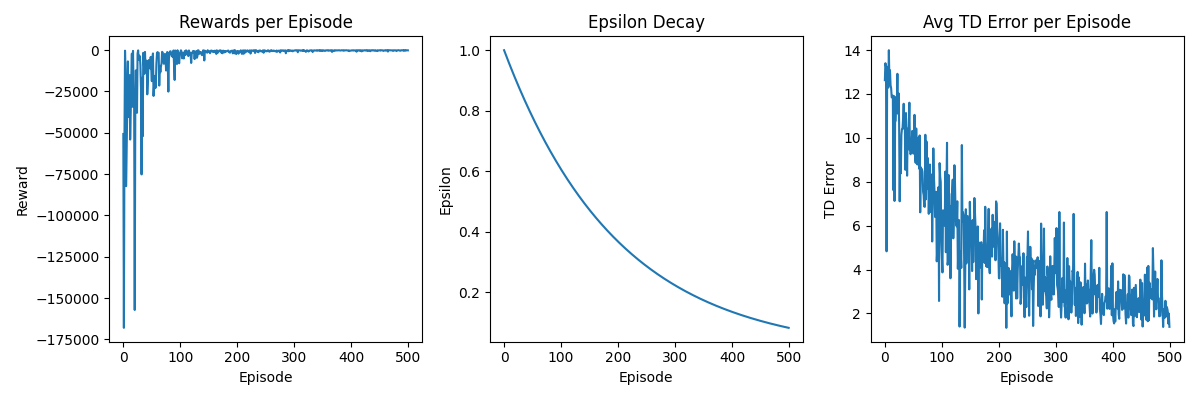
\includegraphics[width=\linewidth]{1_32_0995_64_slip_tab.png}
    \caption{Tabular Q-learning (without random start)}
\end{figure}
\begin{figure}[H]
    \centering
    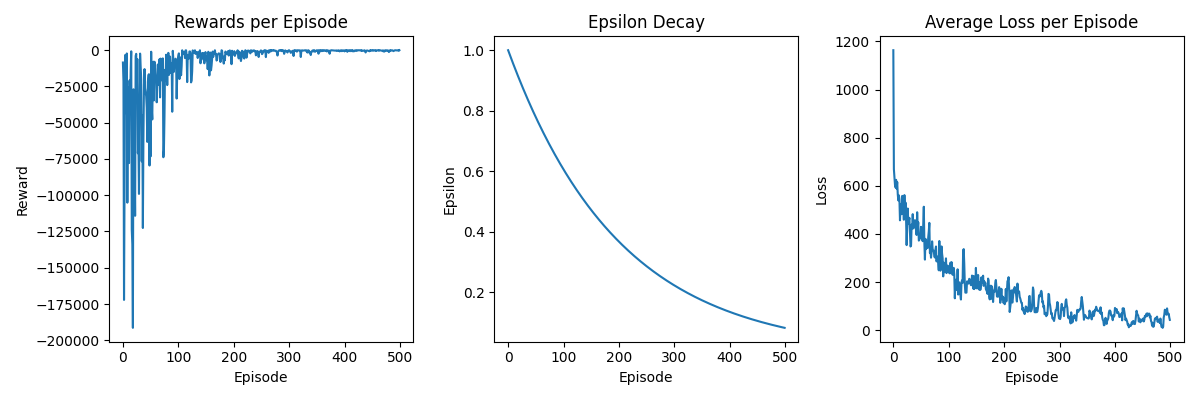
\includegraphics[width=\linewidth]{1_32_0995_64_slip_dqn.png}
    \caption{DQN (without random start)}
\end{figure}
\noindent TABULAR Evaluation Results (over 1000 episodes):
\begin{itemize}
    \item Success Rate: 959/1000 (95.9\%)
    \item Cliff Falls: 0
    \item Avg Total Reward: -69.44
    \item Avg Steps per Episode: 69.44
\end{itemize}
\textbf{DQN} Evaluation Results (over 1000 episodes):
\begin{itemize}
    \item Success Rate: 939/1000 (93.9\%)
    \item Cliff Falls: 158
    \item Avg Total Reward: -92.03
    \item Avg Steps per Episode: 76.39
\end{itemize}
\begin{figure}[H]
    \centering
    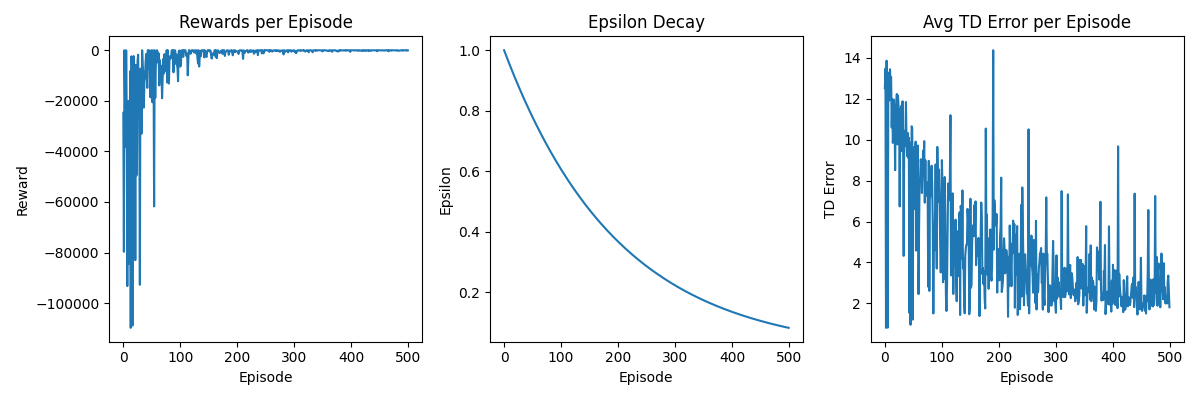
\includegraphics[width=\linewidth]{1_32_0995_64_rand_slip_tab.png}
    \caption{Tabular Q-learning (with random start)}
\end{figure}
\begin{figure}[H]
    \centering
    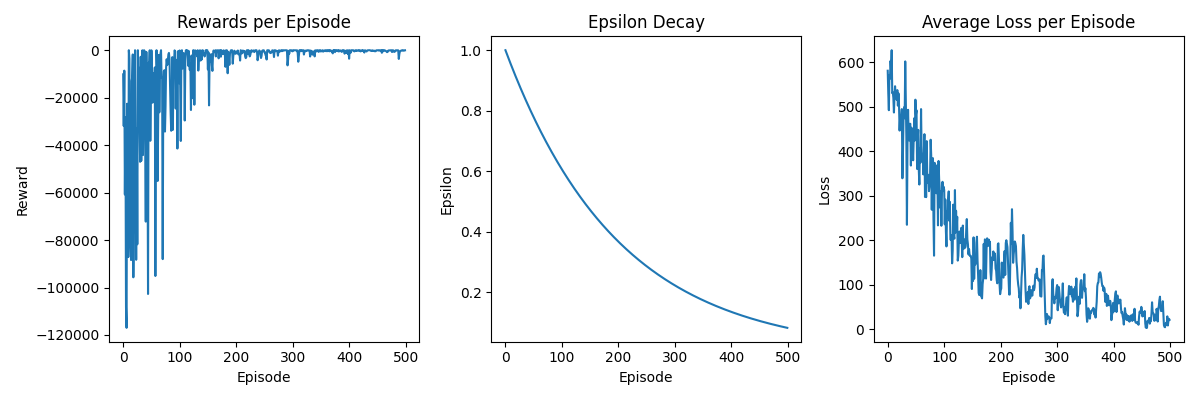
\includegraphics[width=\linewidth]{1_32_0995_64_rand_slip_dqn.png}
    \caption{DQN (with random start)}
\end{figure}
\noindent \textbf{TABULAR} Evaluation Results (over 1000 episodes):
\begin{itemize}
    \item Success Rate: 986/1000 (98.6\%)
    \item Cliff Falls: 0
    \item Avg Total Reward: -45.11
    \item Avg Steps per Episode: 45.11
\end{itemize}
\textbf{DQN} Evaluation Results (over 1000 episodes):
\begin{itemize}
    \item Success Rate: 998/1000 (99.8\%)
    \item Cliff Falls: 0
    \item Avg Total Reward: -70.02
    \item Avg Steps per Episode: 70.02
\end{itemize}
\subsection{Slippery}
The CliffWalking v1 environment has the option to be slippery, adding a probability for each action to cause the agent to move to the wrong position, different from the one associated to the action. 
The slippery option adds nondeterminism but significantly decreases rewards since the agent can randomly deviate from the correct path.

\begin{figure}[H]
    \centering
    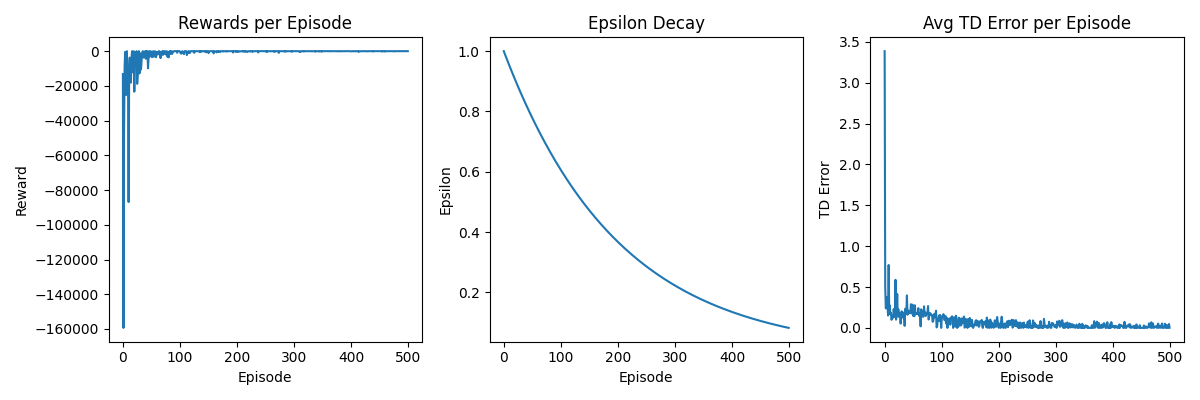
\includegraphics[width=\linewidth]{2_32_0995_64_rand_tab.png}
    \caption{Tabular Q-learning (not slippery)}
\end{figure}
\begin{figure}[H]
    \centering
    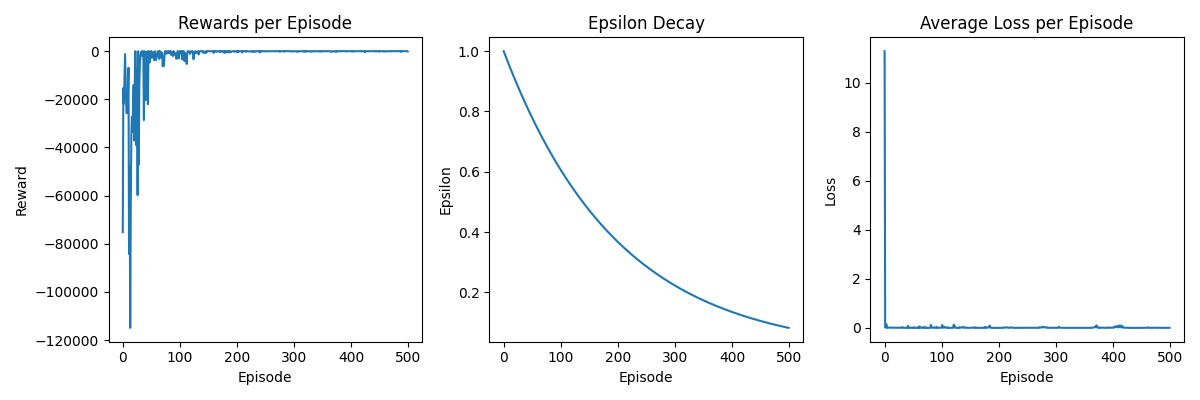
\includegraphics[width=\linewidth]{2_32_0995_64_rand_dqn.png}
    \caption{DQN (not slippery)}
\end{figure}
\noindent \textbf{TABULAR} Evaluation Results (over 1000 episodes):
\begin{itemize}
    \item Success Rate: 1000/1000 (100.0\%)
    \item Cliff Falls: 0
    \item Avg Total Reward: -7.71
    \item Avg Steps per Episode: 7.71
\end{itemize}
\textbf{DQN} Evaluation Results (over 1000 episodes):
\begin{itemize}
    \item Success Rate: 1000/1000 (100.0\%)
    \item Cliff Falls: 0
    \item Avg Total Reward: -7.66
    \item Avg Steps per Episode: 7.66
\end{itemize}


\begin{figure}[H]
    \centering
    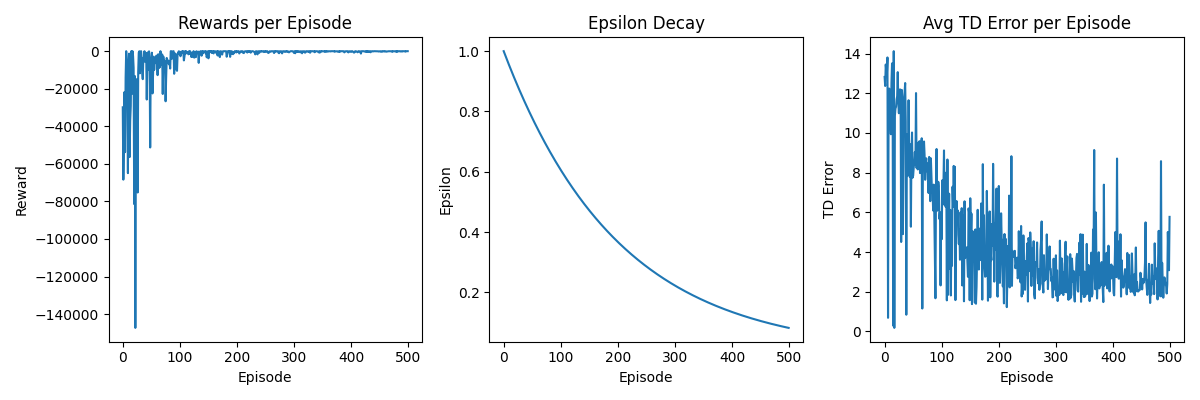
\includegraphics[width=\linewidth]{2_32_0995_64_rand_slip_tab.png}
    \caption{Tabular Q-learning (slippery)}
\end{figure}
\begin{figure}[H]
    \centering
    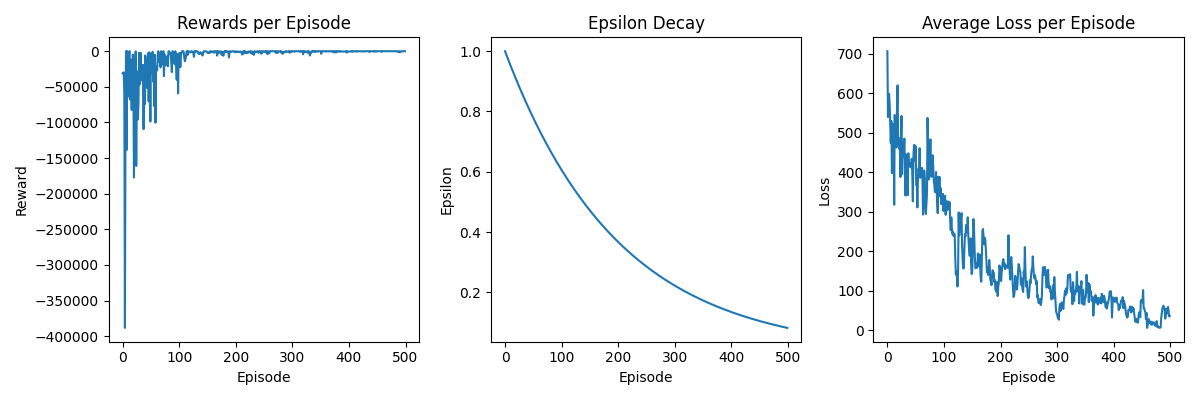
\includegraphics[width=\linewidth]{2_32_0995_64_rand_slip_dqn.png}
    \caption{DQN (slippery)}
\end{figure}
\noindent \textbf{TABULAR} Evaluation Results (over 1000 episodes):
\begin{itemize}
    \item Success Rate: 998/1000 (99.8\%)
    \item Cliff Falls: 0
    \item Avg Total Reward: -44.61
    \item Avg Steps per Episode: 44.61
\end{itemize}
\textbf{DQN} Evaluation Results (over 1000 episodes):
\begin{itemize}
    \item Success Rate: 956/1000 (95.6\%)
    \item Cliff Falls: 0
    \item Avg Total Reward: -88.65
    \item Avg Steps per Episode: 88.65
\end{itemize}

\subsection{Epsilon Decay}
The epsilon value is used in training to balance exploration and exploitation. We always start with $\varepsilon=1$, prioritizing exploration, and decay it over time at a fixed rate to favor exploitation more.\\

\noindent We start with an epsilon decay of 0.995 and can that setting it to 0.999 substantially increases training time and error. Despite that, the agent has a higher chance to find the optimal police due to the fact that exploring is more favored; however, it may waste time exploring wrong paths instead of using the ones it has already found. In our testing, DQN was not able to perform properly with this value.

\begin{figure}[H]
    \centering
    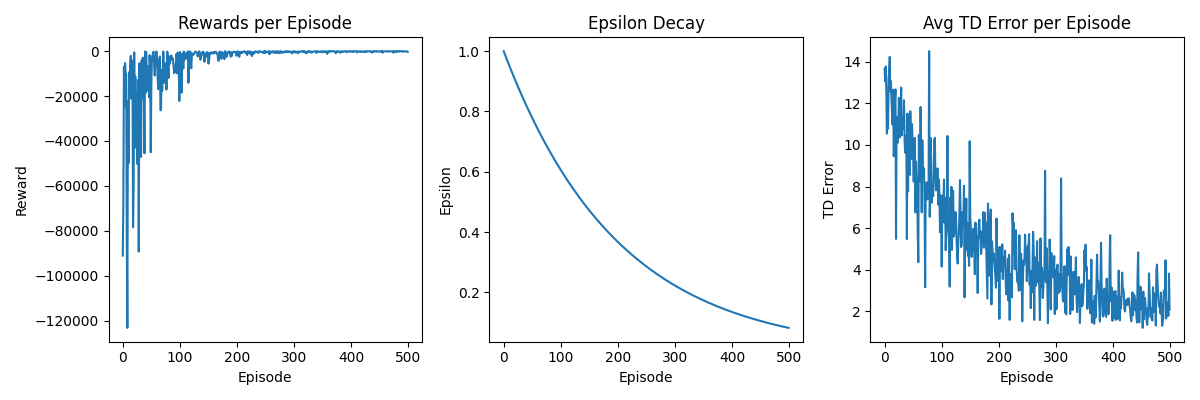
\includegraphics[width=\linewidth]{2_32_0995_64_slip_tab.png}
    \caption{Tabular Q-learning ($\varepsilon$ decay = 0.995)}
\end{figure}
\begin{figure}[H]
    \centering
    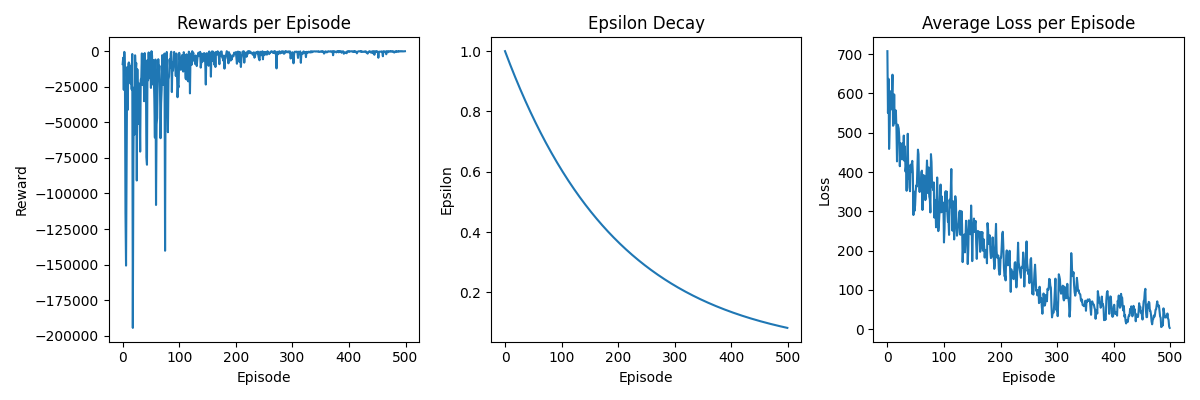
\includegraphics[width=\linewidth]{2_32_0995_64_slip_dqn.png}
    \caption{DQN ($\varepsilon$ decay = 0.995)}
\end{figure}
\noindent \textbf{TABULAR} Evaluation Results (over 1000 episodes):
\begin{itemize}
    \item Success Rate: 946/1000 (94.6\%)
    \item Cliff Falls: 0
    \item Avg Total Reward: -77.27
    \item Avg Steps per Episode: 77.27
\end{itemize}
\textbf{DQN} Evaluation Results (over 1000 episodes):
\begin{itemize}
    \item Success Rate: 931/1000 (93.1\%)
    \item Cliff Falls: 0
    \item Avg Total Reward: -83.50
    \item Avg Steps per Episode: 83.50
\end{itemize}


\begin{figure}[H]
    \centering
    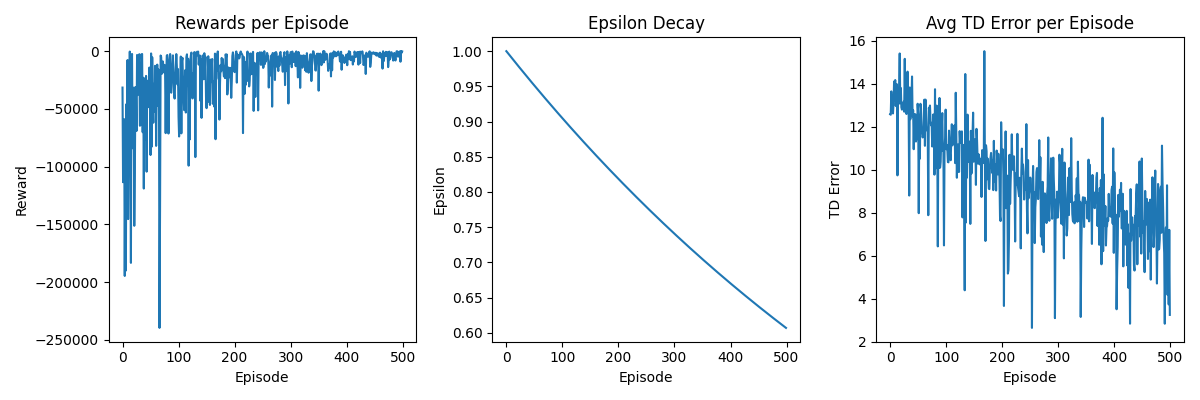
\includegraphics[width=\linewidth]{2_32_0999_64_slip_tab.png}
    \caption{Tabular Q-learning ($\varepsilon$ decay = 0.999)}
\end{figure}
\begin{figure}[H]
    \centering
    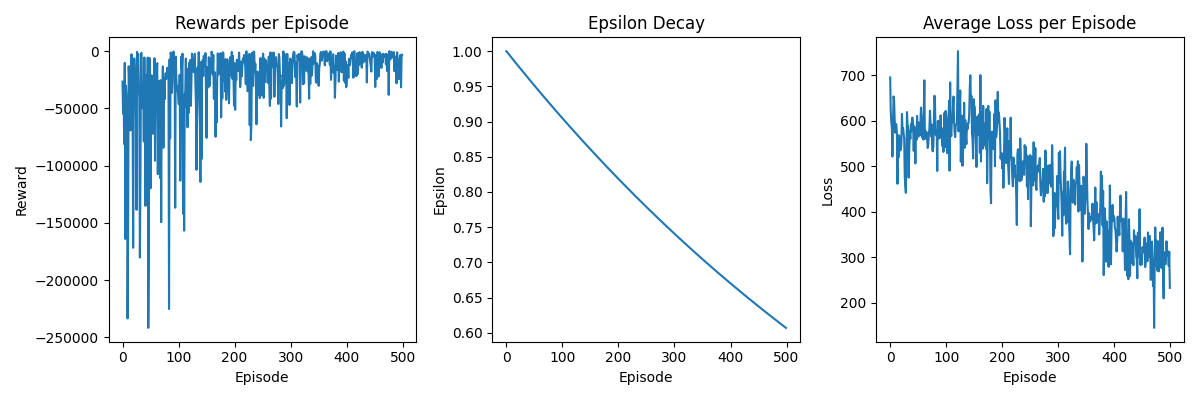
\includegraphics[width=\linewidth]{2_32_0999_64_slip_dqn.png}
    \caption{DQN ($\varepsilon$ decay = 0.999)}
\end{figure}
\noindent \textbf{TABULAR} Evaluation Results (over 1000 episodes):
\begin{itemize}
    \item Success Rate: 942/1000 (94.2\%)
    \item Cliff Falls: 0
    \item Avg Total Reward: -82.18
    \item Avg Steps per Episode: 82.18
\end{itemize}
\textbf{DQN} Evaluation Results (over 1000 episodes):
\begin{itemize}
    \item Success Rate: 0/1000 (0.0\%)
    \item Cliff Falls: 0
    \item Avg Total Reward: -358.43
    \item Avg Steps per Episode: 358.43
\end{itemize}

\noindent When instead we reduce the epsilon decay, we favor exploitation more, exploring less paths. This can lead to the agent missing potential new paths that are better in favor of using the ones it has already explored. In our testing this can be seen in a lower average reward when we reduce the epsilon decay from 0.995 to 0.99.
\begin{figure}[H]
    \centering
    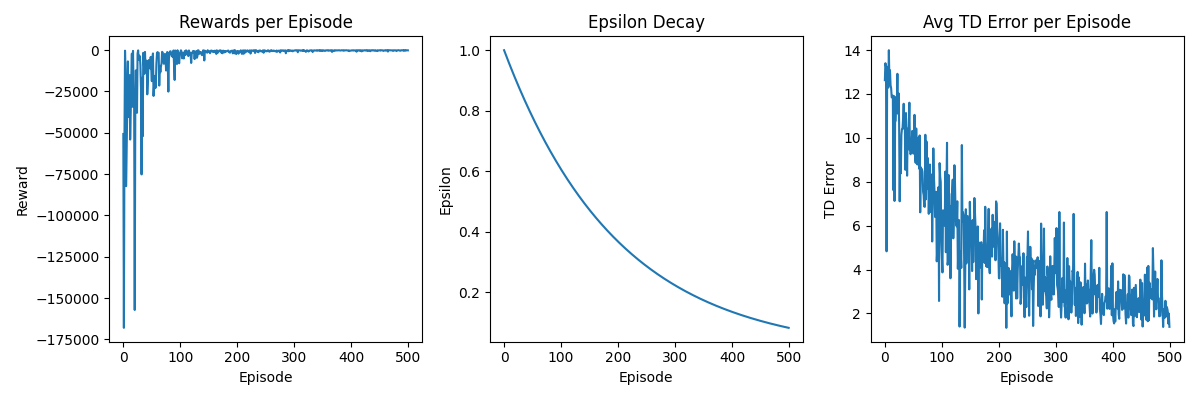
\includegraphics[width=\linewidth]{1_32_0995_64_slip_tab.png}
    \caption{Tabular Q-learning ($\varepsilon$ decay = 0.995)}
\end{figure}
\begin{figure}[H]
    \centering
    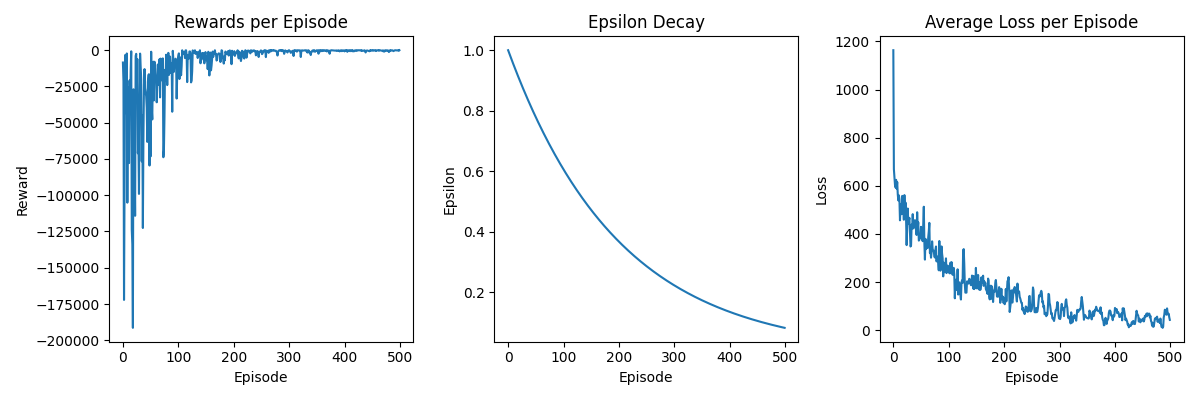
\includegraphics[width=\linewidth]{1_32_0995_64_slip_dqn.png}
    \caption{DQN ($\varepsilon$ decay = 0.995)}
\end{figure}
\noindent \textbf{TABULAR} Evaluation Results (over 1000 episodes):
\begin{itemize}
    \item Success Rate: 959/1000 (95.9\%)
    \item Cliff Falls: 0
    \item Avg Total Reward: -69.44
    \item Avg Steps per Episode: 69.44
\end{itemize}
\textbf{DQN} Evaluation Results (over 1000 episodes):
\begin{itemize}
    \item Success Rate: 939/1000 (93.9\%)
    \item Cliff Falls: 158
    \item Avg Total Reward: -92.03
    \item Avg Steps per Episode: 76.39
\end{itemize}


\begin{figure}[H]
    \centering
    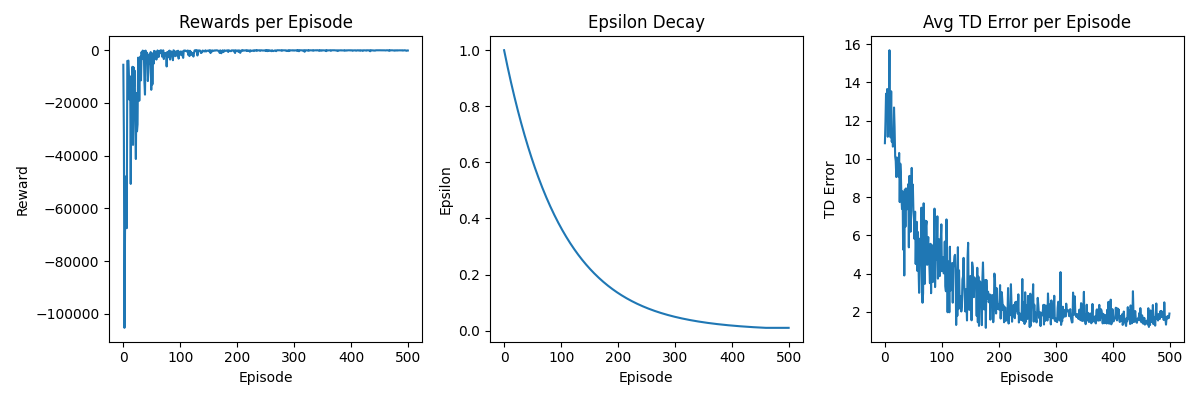
\includegraphics[width=\linewidth]{1_32_099_64_slip_tab.png}
    \caption{Tabular Q-learning ($\varepsilon$ decay = 0.99)}
\end{figure}
\begin{figure}[H]
    \centering
    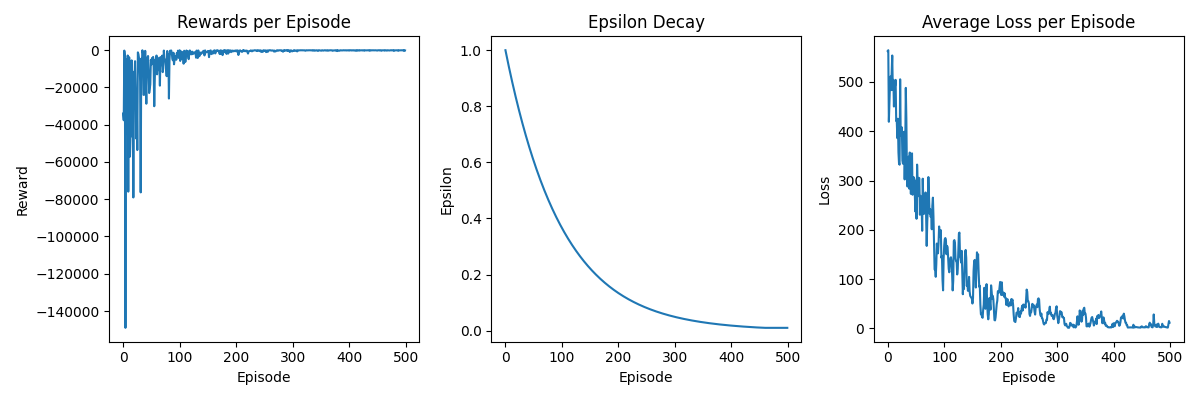
\includegraphics[width=\linewidth]{1_32_099_64_slip_dqn.png}
    \caption{DQN ($\varepsilon$ decay = 0.99)}
\end{figure}
\noindent \textbf{TABULAR} Evaluation Results (over 1000 episodes):
\begin{itemize}
    \item Success Rate: 950/1000 (95.0\%)
    \item Cliff Falls: 0
    \item Avg Total Reward: -68.81
    \item Avg Steps per Episode: 68.81
\end{itemize}
\textbf{DQN} Evaluation Results (over 1000 episodes):
\begin{itemize}
    \item Success Rate: 926/1000 (92.6\%)
    \item Cliff Falls: 467
    \item Avg Total Reward: -128.62
    \item Avg Steps per Episode: 82.39
\end{itemize}



\subsection{Training Episodes}
The number of episodes used for training should be large enough for the agent to reach the goal. If this number is too small, the agent may get stuck in a loop and thus never reach the goal. This is more evident in DQN, since the network needs more training to perform efficiently compared to tabular Q-learning.\\

\noindent We used 500 episodes for the majority of the training but we also tried lower numbers. When trained over a small number of episodes, DQN gives inconsistent results between different trainings, often achieving a very low success rate while sometimes getting better scores.\\

\begin{figure}[H]
    \centering
    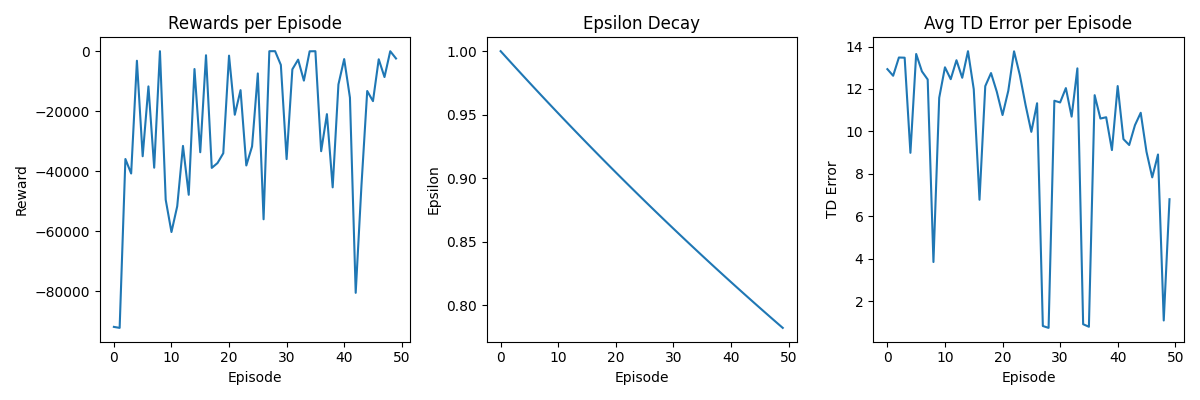
\includegraphics[width=\linewidth]{plot_tabular_50ep.png}
    \caption{Tabular Q-learning (50 episodes)}
\end{figure}
\begin{figure}[H]
    \centering
    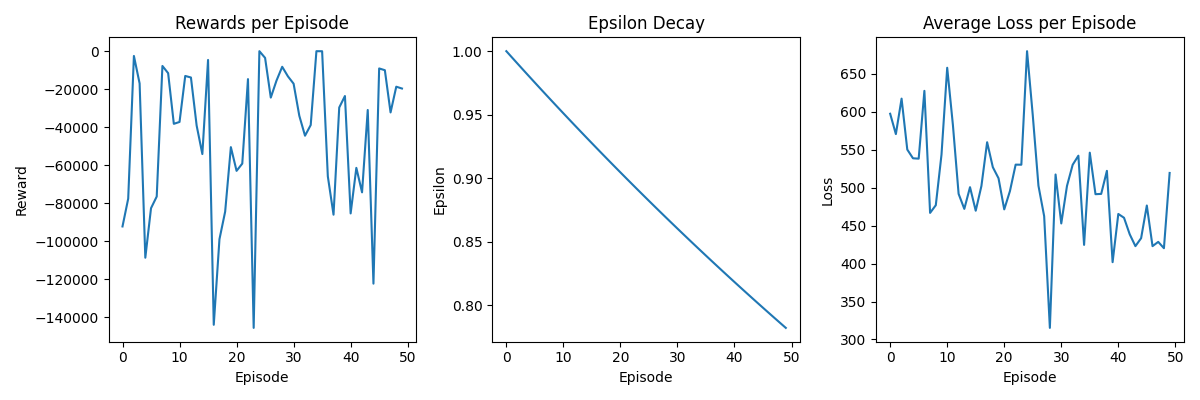
\includegraphics[width=\linewidth]{plot_dqn_50ep.png}
    \caption{DQN (50 episodes)}
\end{figure}
\noindent \textbf{TABULAR} Evaluation Results (over 1000 episodes):
\begin{itemize}
    \item Success Rate: 956/1000 (95.6\%)
    \item Cliff Falls: 0
    \item Avg Total Reward: -49.27
    \item Avg Steps per Episode: 49.27
\end{itemize}
\textbf{DQN} Evaluation Results (over 1000 episodes):
\begin{itemize}
    \item Success Rate: 0/1000 (0.0\%)
    \item Cliff Falls: 1609
    \item Avg Total Reward: -520.71
    \item Avg Steps per Episode:361.42
\end{itemize}


\begin{figure}[H]
    \centering
    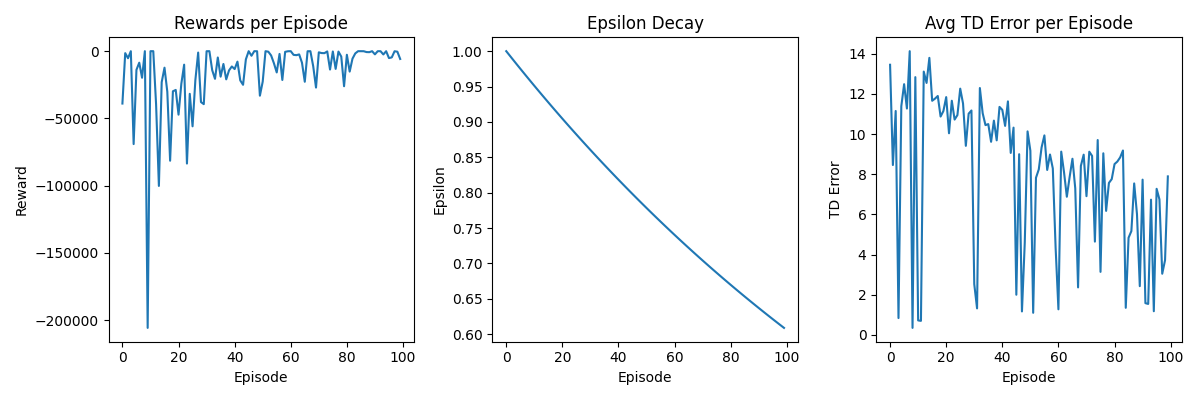
\includegraphics[width=\linewidth]{plot_tabular_100ep.png}
    \caption{Tabular Q-learning (100 episodes)}
\end{figure}
\begin{figure}[H]
    \centering
    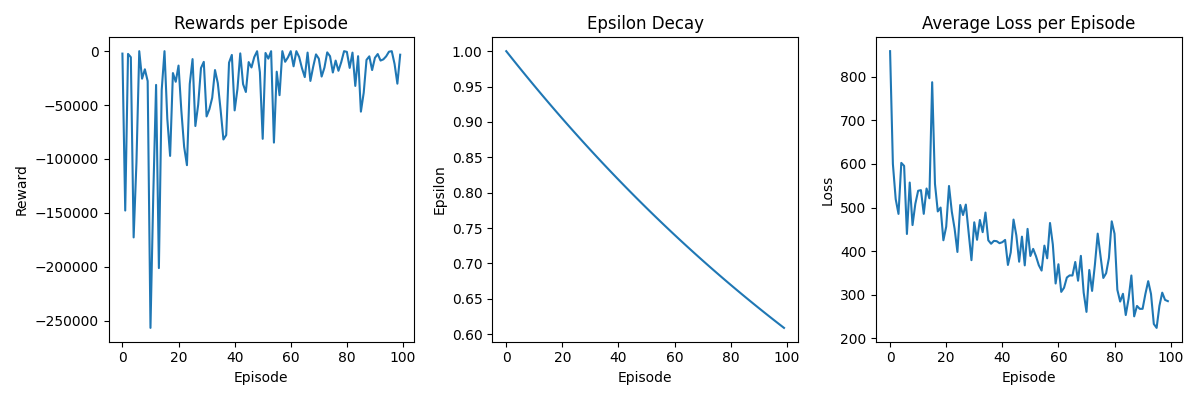
\includegraphics[width=\linewidth]{plot_dqn_100ep.png}
    \caption{DQN (100 episodes)}
\end{figure}
\noindent \textbf{TABULAR} Evaluation Results (over 1000 episodes):
\begin{itemize}
    \item Success Rate: 963/1000 (96.3\%)
    \item Cliff Falls: 0
    \item Avg Total Reward: -45.41
    \item Avg Steps per Episode: 45.41
\end{itemize}
\textbf{DQN} Evaluation Results (over 1000 episodes):
\begin{itemize}
    \item Success Rate: 984/1000 (98.4\%)
    \item Cliff Falls: 0
    \item Avg Total Reward: -92.77
    \item Avg Steps per Episode: 92.77
\end{itemize}

\begin{figure}[H]
    \centering
    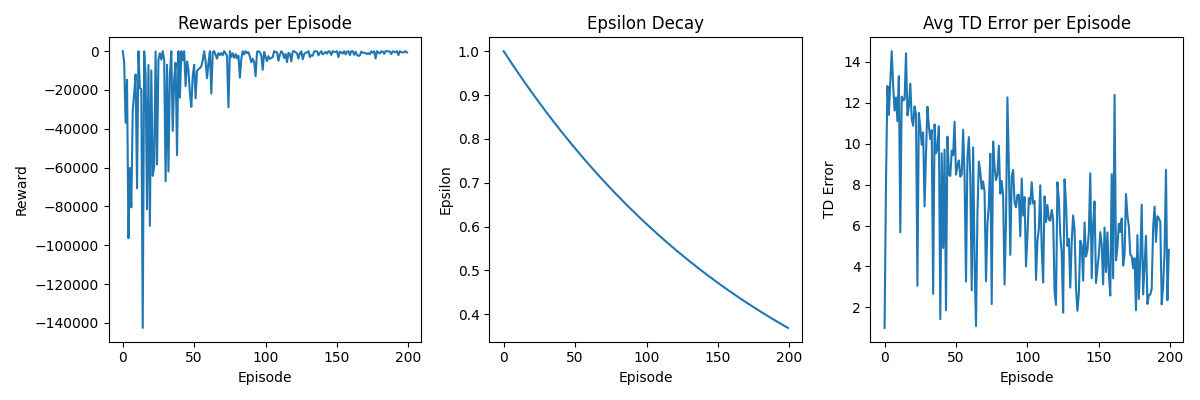
\includegraphics[width=\linewidth]{plot_tabular_200ep.png}
    \caption{Tabular Q-learning (200 episodes)}
\end{figure}
\begin{figure}[H]
    \centering
    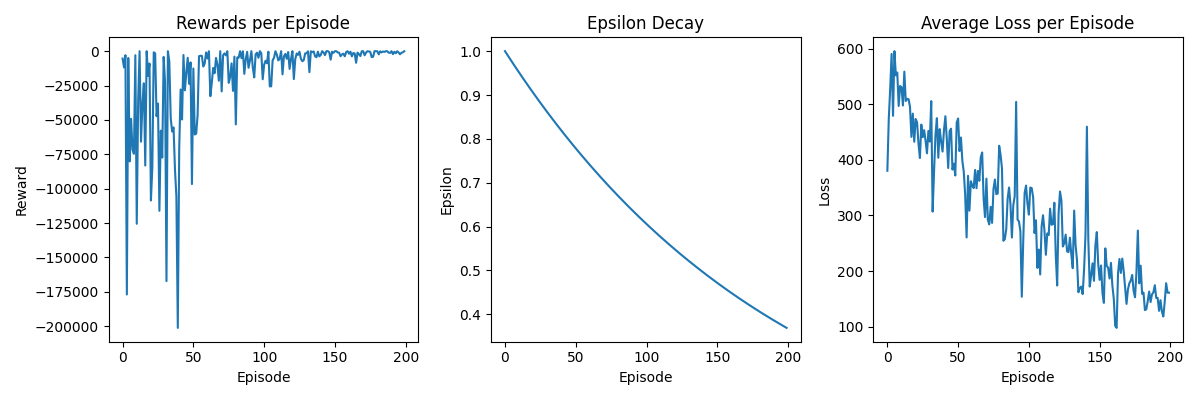
\includegraphics[width=\linewidth]{plot_dqn200ep.png}
    \caption{DQN (200 episodes)}
\end{figure}
\noindent \textbf{TABULAR} Evaluation Results (over 1000 episodes):
\begin{itemize}
    \item Success Rate: 965/1000 (96.5\%)
    \item Cliff Falls: 0
    \item Avg Total Reward: -45.64
    \item Avg Steps per Episode: 45.64
\end{itemize}
\textbf{DQN} Evaluation Results (over 1000 episodes):
\begin{itemize}
    \item Success Rate: 861/1000 (86.1\%)
    \item Cliff Falls: 395
    \item Avg Total Reward: -144.46
    \item Avg Steps per Episode: 105.36
\end{itemize}

\noindent Obviously, since DQN is much more powerful, it should perform better in more complex environments despite the need to be trained for more episodes.

\subsection{Hidden Layers and Neurons}
The neural network used for DQN can be configured in terms of the number of hidden layers and neurons per layer.
We started with a base consisting of 2 hidden layers of 32 neurons and tweaked both numbers to observe the difference in the results.\\
\begin{figure}[H]
    \centering
    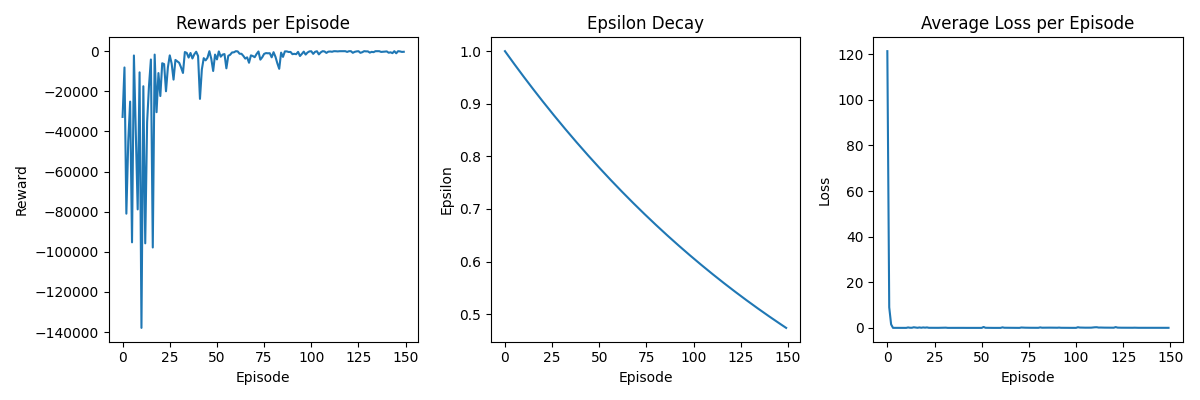
\includegraphics[width=\linewidth]{1_16.png}
    \caption{DQN training with 1 hidden layer and 16 neurons}
\end{figure}
\textbf{DQN} Evaluation Results (over 1000 episodes):
\begin{itemize}
    \item Success Rate: 0/1000 (0.0\%)
    \item Cliff Falls: 0
    \item Avg Total Reward: -17.00
    \item Avg Steps per Episode: 17.00
\end{itemize}
\begin{figure}[H]
    \centering
    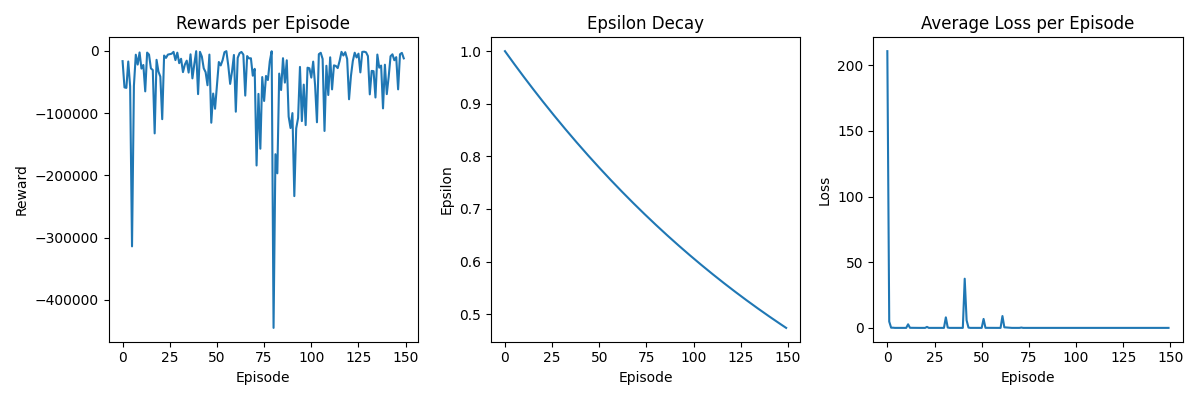
\includegraphics[width=\linewidth]{1_32.png}
    \caption{DQN training with 1 hidden layer and 32 neurons}
\end{figure}
\textbf{DQN} Evaluation Results (over 1000 episodes):
\begin{itemize}
    \item Success Rate: 0/1000 (0.0\%)
    \item Cliff Falls: 0
    \item Avg Total Reward: -11.00
    \item Avg Steps per Episode: 11.00
\end{itemize}
\begin{figure}[H]
    \centering
    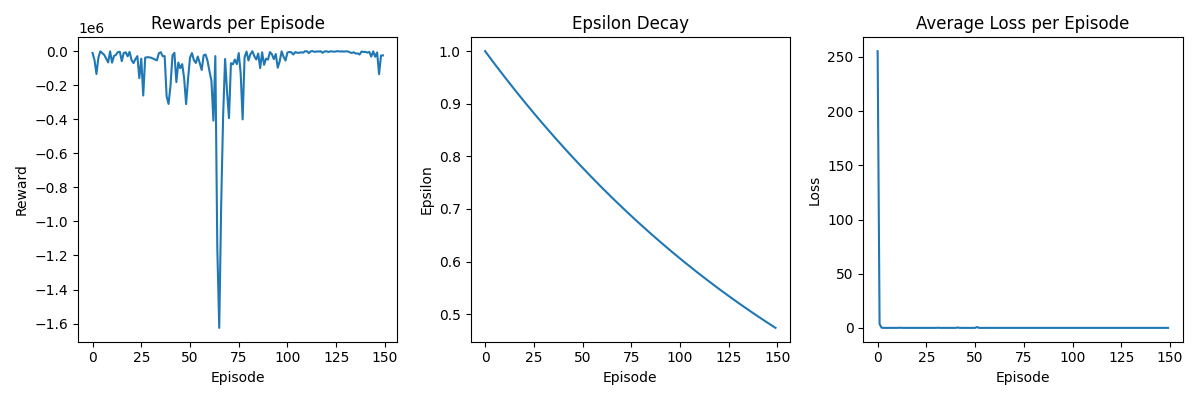
\includegraphics[width=\linewidth]{1_64.png}
    \caption{DQN training with 1 hidden layer and 64 neurons}
\end{figure}
\textbf{DQN} Evaluation Results (over 1000 episodes):
\begin{itemize}
    \item Success Rate: 0/1000 (0.0\%)
    \item Cliff Falls: 0
    \item Avg Total Reward: -11.00
    \item Avg Steps per Episode: 11.00
\end{itemize}
\begin{figure}[H]
    \centering
    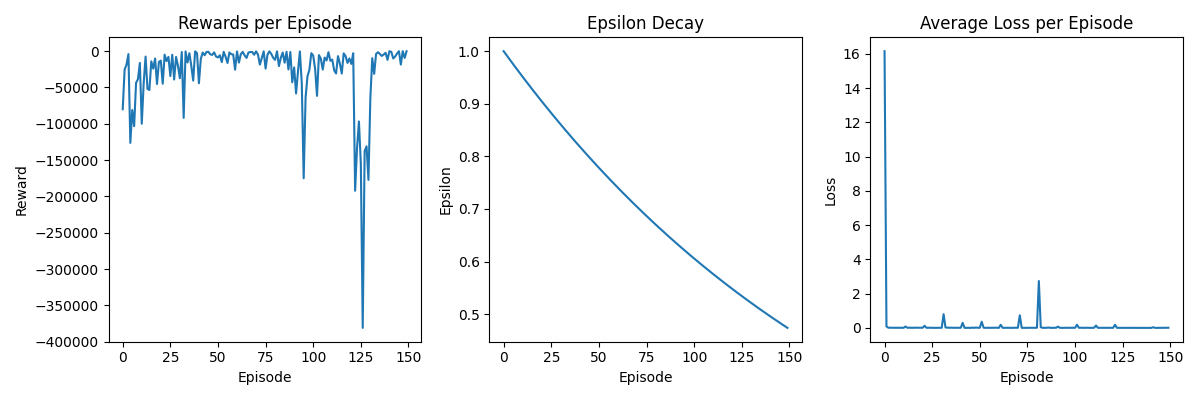
\includegraphics[width=\linewidth]{1_128.png}
    \caption{DQN training with 1 hidden layer and 128 neurons}
\end{figure}
\textbf{DQN} Evaluation Results (over 1000 episodes):
\begin{itemize}
    \item Success Rate: 0/1000 (0.0\%)
    \item Cliff Falls: 0
    \item Avg Total Reward: -11.00
    \item Avg Steps per Episode: 11.00
\end{itemize}
\begin{figure}[H]
    \centering
    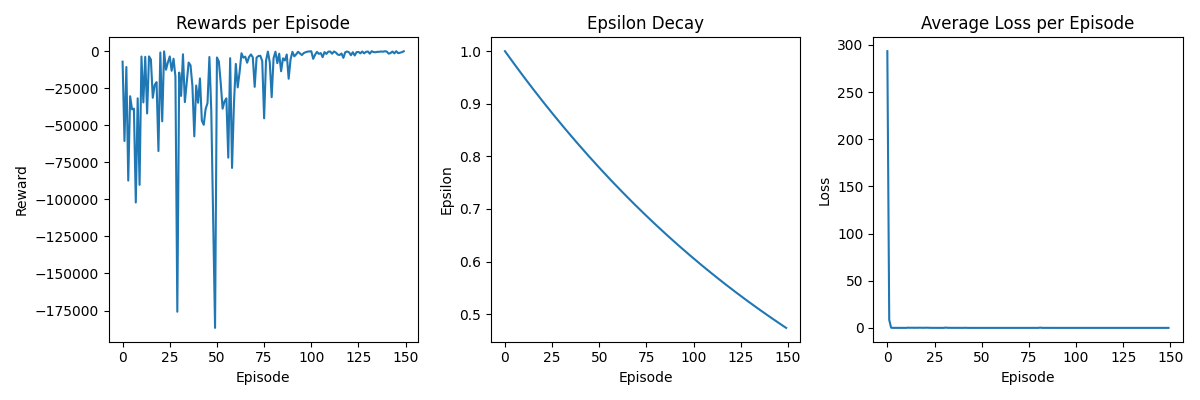
\includegraphics[width=\linewidth]{2_16.png}
    \caption{DQN training with 2 hidden layer and 16 neurons}
\end{figure}
\textbf{DQN} Evaluation Results (over 1000 episodes):
\begin{itemize}
    \item Success Rate: 0/1000 (0.0\%)
    \item Cliff Falls: 0
    \item Avg Total Reward: -11.00
    \item Avg Steps per Episode: 11.00
\end{itemize}
\begin{figure}[H]
    \centering
    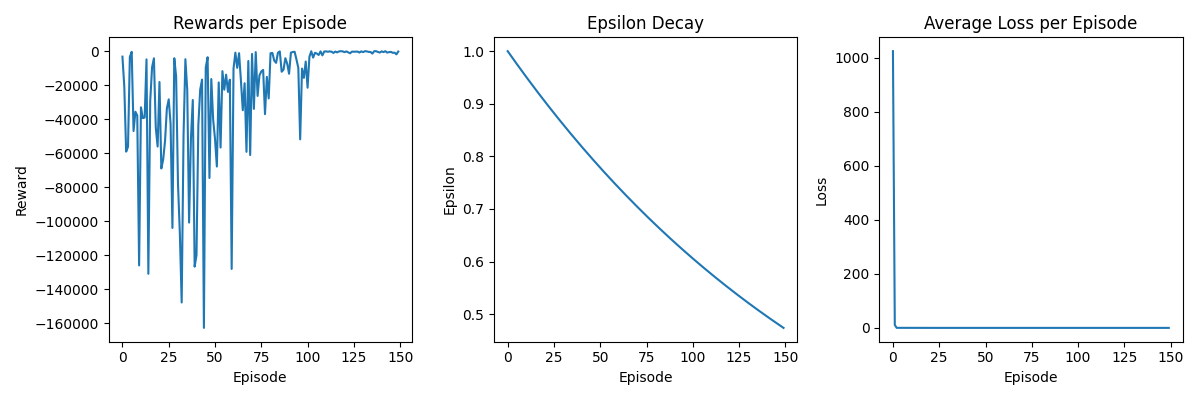
\includegraphics[width=\linewidth]{2_32.png}
    \caption{DQN training with 2 hidden layer and 32 neurons}
\end{figure}
\textbf{DQN} Evaluation Results (over 1000 episodes):
\begin{itemize}
    \item Success Rate: 1000/1000 (100.0\%)
    \item Cliff Falls: 0
    \item Avg Total Reward: -13.00
    \item Avg Steps per Episode: 13.00
\end{itemize}
\begin{figure}[H]
    \centering
    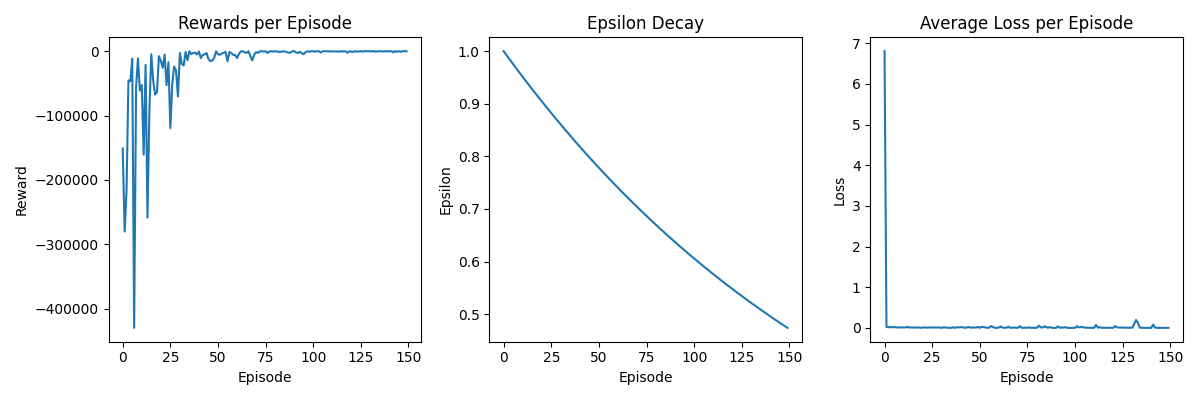
\includegraphics[width=\linewidth]{2_64.png}
    \caption{DQN training with 2 hidden layer and 64 neurons}
\end{figure}
\textbf{DQN} Evaluation Results (over 1000 episodes):
\begin{itemize}
    \item Success Rate: 1000/1000 (100.0\%)
    \item Cliff Falls: 0
    \item Avg Total Reward: -13.00
    \item Avg Steps per Episode: 13.00
\end{itemize}
\begin{figure}[H]
    \centering
    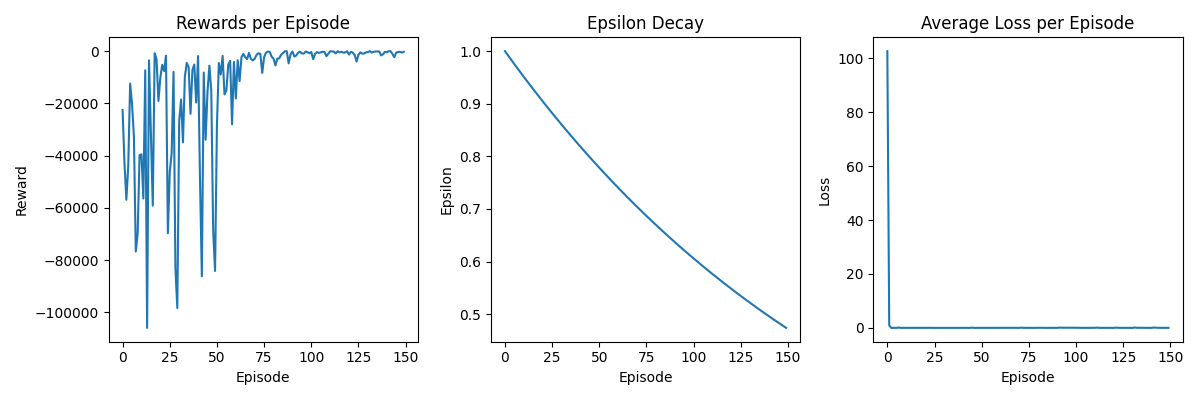
\includegraphics[width=\linewidth]{3_16.png}
    \caption{DQN training with 3 hidden layer and 16 neurons}
\end{figure}
\textbf{DQN} Evaluation Results (over 1000 episodes):
\begin{itemize}
    \item Success Rate: 1000/1000 (100.0\%)
    \item Cliff Falls: 0
    \item Avg Total Reward: -13.00
    \item Avg Steps per Episode: 13.00
\end{itemize}
\vspace{0,5cm}
As we can see from the graphs, it is more convenient to increase depth instead of width to improve the performance of the DQN. We can't reach the performance of the "2 hidden layers and 32 neurons" DQN with just 1 hidden layer, even by increasing the number of neurons to 128, but we can easily match it with 3 hidden layers and just 16 neurons. This confirms that, in practice, a deep and narrow network is easier to train and provides
better results in generalization.

\section{Conclusions}
In this project we have implemented tabular Q-learning and DQN to perform Reinforcement Learning in the Cliff Walking environment. We have tested the two approaches and put them side by side, comparing their performance in this environment. We have reached the conclusion that, in the Cliff Walking environment, DQN is often slower and noisier compared to tabular Q-learning. This is because the environment has a small space state and the agent doesn't need the power of a neural network since the Q table can be easily computed. In bigger and more complex environments, however, it is expected that DQN would perform much better than tabular Q-learning since, with a much higher number of states, the Q table would become much larger and slow down performance.\\

\noindent So, in conclusion, both approaches have their strengths and weaknesses, with tabular Q-learning being preferred for simpler and smaller environments and DQN favoring larger and more complex ones. The key insight is that algorithm selection must carefully consider problem characteristics, computational constraints and performance requirements rather than defaulting to the most sophisticated available method.
\end{document}